% $Id: template.tex 11 2007-04-03 22:25:53Z jpeltier $

\documentclass{vgtc}                          % final (conference style)
%\documentclass[review]{vgtc}                 % review
%\documentclass[widereview]{vgtc}             % wide-spaced review
%\documentclass[preprint]{vgtc}               % preprint
%\documentclass[electronic]{vgtc}             % electronic version

%% Uncomment one of the lines above depending on where your paper is
%% in the conference process. ``review'' and ``widereview'' are for review
%% submission, ``preprint'' is for pre-publication, and the final version
%% doesn't use a specific qualifier. Further, ``electronic'' includes
%% hyperreferences for more convenient online viewing.

%% Please use one of the ``review'' options in combination with the
%% assigned online id (see below) ONLY if your paper uses a double blind
%% review process. Some conferences, like IEEE Vis and InfoVis, have NOT
%% in the past.

%% Figures should be in CMYK or Grey scale format, otherwise, colour
%% shifting may occur during the printing process.

%% These few lines make a distinction between latex and pdflatex calls and they
%% bring in essential packages for graphics and font handling.
%% Note that due to the \DeclareGraphicsExtensions{} call it is no longer necessary
%% to provide the the path and extension of a graphics file:
%% \includegraphics{diamondrule} is completely sufficient.
%%
\ifpdf%                                % if we use pdflatex
  \pdfoutput=1\relax                   % create PDFs from pdfLaTeX
  \pdfcompresslevel=9                  % PDF Compression
  \pdfoptionpdfminorversion=7          % create PDF 1.7
  \ExecuteOptions{pdftex}
  \usepackage{graphicx}                % allow us to embed graphics files
  \DeclareGraphicsExtensions{.pdf,.png,.jpg,.jpeg} % for pdflatex we expect .pdf, .png, or .jpg files
\else%                                 % else we use pure latex
  \ExecuteOptions{dvips}
  \usepackage{graphicx}                % allow us to embed graphics files
  \DeclareGraphicsExtensions{.eps}     % for pure latex we expect eps files
\fi%

%% it is recomended to use ``\autoref{sec:bla}'' instead of ``Fig.~\ref{sec:bla}''
\graphicspath{{figures/}{pictures/}{images/}{./}} % where to search for the images

\usepackage{microtype}                 % use micro-typography (slightly more compact, better to read)
\PassOptionsToPackage{warn}{textcomp}  % to address font issues with \textrightarrow
\usepackage{textcomp}                  % use better special symbols
\usepackage{mathptmx}                  % use matching math font
\usepackage{times}                     % we use Times as the main font
\renewcommand*\ttdefault{txtt}         % a nicer typewriter font
\usepackage{cite}                      % needed to automatically sort the references
\usepackage{tabu}                      % only used for the table example
\usepackage{booktabs}                  % only used for the table example
%% We encourage the use of mathptmx for consistent usage of times font
%% throughout the proceedings. However, if you encounter conflicts
%% with other math-related packages, you may want to disable it.


%% If you are submitting a paper to a conference for review with a double
%% blind reviewing process, please replace the value ``0'' below with your
%% OnlineID. Otherwise, you may safely leave it at ``0''.
\onlineid{0}

%% declare the category of your paper, only shown in review mode
\vgtccategory{Research}

%% allow for this line if you want the electronic option to work properly
\vgtcinsertpkg

%% In preprint mode you may define your own headline.
%\preprinttext{To appear in an IEEE VGTC sponsored conference.}

%% Paper title.

\title{OPTICSvis: Visualizing the OPTICS algorithm}

%% This is how authors are specified in the conference style

%% Author and Affiliation (single author).
%%\author{Roy G. Biv\thanks{e-mail: roy.g.biv@aol.com}}
%%\affiliation{\scriptsize Allied Widgets Research}

%% Author and Affiliation (multiple authors with single affiliations).
%%\author{Roy G. Biv\thanks{e-mail: roy.g.biv@aol.com} %
%%\and Ed Grimley\thanks{e-mail:ed.grimley@aol.com} %
%%\and Martha Stewart\thanks{e-mail:martha.stewart@marthastewart.com}}
%%\affiliation{\scriptsize Martha Stewart Enterprises \\ Microsoft Research}

%% Author and Affiliation (multiple authors with multiple affiliations)
\author{Sonja Biedermann\thanks{e-mail:sonja.biedermann@univie.ac.at }\\ %
        \scriptsize University of Vienna %
\and Christian Permann\thanks{e-mail:a01463926@unet.univie.ac.at}\\ %
     \scriptsize  University of Vienna}

%% A teaser figure can be included as follows, but is not recommended since
%% the space is now taken up by a full width abstract.
%\teaser{
%  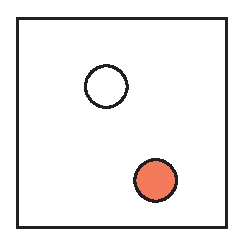
\includegraphics[width=1.5in]{sample.eps}
%  \caption{Lookit! Lookit!}
%}

%% Abstract section.
\abstract{Duis autem vel eum iriure dolor in hendrerit in vulputate
velit esse molestie consequat, vel illum dolore eu feugiat nulla
facilisis at vero eros et accumsan et iusto odio dignissim qui blandit
praesent luptatum zzril delenit augue duis dolore te feugait nulla
facilisi. Lorem ipsum dolor sit amet, consectetuer adipiscing elit,
sed diam nonummy nibh euismod tincidunt ut laoreet dolore magna
aliquam erat volutpat. Ut wisi enim ad minim veniam, quis nostrud exerci tation ullamcorper
suscipit lobortis nisl ut aliquip ex ea commodo consequat. Duis autem
vel eum iriure dolor in hendrerit in vulputate velit esse molestie
consequat, vel illum dolore eu feugiat nulla facilisis at vero eros et
accumsan et iusto odio dignissim qui blandit praesent luptatum zzril
delenit augue duis dolore te feugait nulla facilisi.%
} % end of abstract

%% ACM Computing Classification System (CCS).
%% See <http://www.acm.org/about/class> for details.
%% We recommend the 2012 system <http://www.acm.org/about/class/class/2012>
%% For the 2012 system use the ``\CCScatTwelve'' which command takes four arguments.
%% The 1998 system <http://www.acm.org/about/class/class/2012> is still possible
%% For the 1998 system use the ``\CCScat'' which command takes four arguments.
%% In both cases the last two arguments (1998) or last three (2012) can be empty.

\CCScatlist{
  \CCScatTwelve{Human-centered computing}{Visu\-al\-iza\-tion}{Visu\-al\-iza\-tion techniques}{Treemaps};
  \CCScatTwelve{Human-centered computing}{Visu\-al\-iza\-tion}{Visualization design and evaluation methods}{}
}

%\CCScatlist{
  %\CCScat{H.5.2}{User Interfaces}{User Interfaces}{Graphical user interfaces (GUI)}{};
  %\CCScat{H.5.m}{Information Interfaces and Presentation}{Miscellaneous}{}{}
%}

%% Copyright space is enabled by default as required by guidelines.
%% It is disabled by the 'review' option or via the following command:
% \nocopyrightspace

%%%%%%%%%%%%%%%%%%%%%%%%%%%%%%%%%%%%%%%%%%%%%%%%%%%%%%%%%%%%%%%%
%%%%%%%%%%%%%%%%%%%%%% START OF THE PAPER %%%%%%%%%%%%%%%%%%%%%%
%%%%%%%%%%%%%%%%%%%%%%%%%%%%%%%%%%%%%%%%%%%%%%%%%%%%%%%%%%%%%%%%%

\begin{document}
%% The ``\maketitle'' command must be the first command after the
%% ``\begin{document}'' command. It prepares and prints the title block.

%% the only exception to this rule is the \firstsection command
\firstsection{Introduction} % sonja

\maketitle

%% \section{Introduction} %for journal use above \firstsection{..} instead

\begin{flushleft}
The OPTICS algorithm is a density based clustering algorithm, that outputs a list of points,
 ordered according to the reachability of the points and the logic of the algorithm.
This result is usually visualized by plotting this list as a bar chart with the output index as x-value and the
computed reachability distance as y-value. This reachability plot then is used to make assumptions about
the cluster-hierarchy in the data.
\end{flushleft}

\begin{flushleft}
Our project idea is to visualize the resulting data from running the OPTICS algorithm on a given data set. OPTICS does not generate a simple mapping of points to a cluster ID, but rather outputs a list of reachability data - that is, the length (given by, e.g., the euclidean distance between those two points) that the algorithm had to jump from a given point to another. Short distances are preferred by the algorithm, so a series of short jumps likely marks a cluster.
\end{flushleft}

\begin{flushleft}
However, in the end the user is looking at nothing but numbers and has to discern the patterns in the data himself. As such, the first step after running OPTICS is usually to draw a bar chart, which makes this task much easier.
\end{flushleft}

\begin{flushleft}
As such, visualization is arguably already a core component of cluster analysis when using OPTICS. Why not allow for further manipulation of the algorithm, allowing to specify parameters such as the minimum point size to qualifiy as a cluster, or the cutoff distance that is applied onto the reachability data to define the actual clusters?
\end{flushleft}

\begin{flushleft}
Furthermore, OPTICS is inherently capable of producing hierarchial clusterings, but this information is oftentimes discarded in favor of a simpler representation. Procuring an visualization method that is still simple, but allows for evaluation of hierarchial clusters is surely a worthwile undertaking, and one that we will strive for.
\end{flushleft}

\section{Motivation} %% sonja

\begin{flushleft}
 Not many tools exist that take on this subject, although notable projects exist, especially Clustervision\cite{Clustervision} and a DBSCAN visualization that we found \cite{DBSCAN}, the latter of which only visualizes how DBSCAN goes about finding clusters (i.e. shows the epsilon neighborhoods). It is notable that DBSCAN results in a simple partition of points into clusters along with some metadata (e.g. core points versus edge points).
\end{flushleft}

\begin{flushleft}
Clustervision is an especially powerful tool and takes on a multitude of algorithms (including OPTICS) and offers additional tooling like dimension reduction using TSNE. One of the core tasks of this tool is to validate the results of the algorithm - i.e. enable the user to check out the features of points in a cluster and see the relations between data that caused them to be classified into the same cluster.
\end{flushleft}

\begin{flushleft}
This is something that we do not want to do, as we strongly feel that this is out of bounds for us. We want to make an example of simple data (i.e. low dimensional and spatial, a list of real points) and how the results given by OPTICS relate to this data set and the used settings, and show the partition derived from the reachability data.
\end{flushleft}

\subsection{Background information}
\subsubsection{Users}
\begin{itemize}
\item Teachers and Students
\item Researchers
\item Anyone interested in the OPTICS algorithm
\end{itemize}
\subsubsection{Tasks}
\begin{flushleft}
The main task our implementation aims to help with, is to educate on how use OPTICS and to see if it fits given data and problem.
\end{flushleft}

\begin{flushleft}
Teachers can either use our default data set or load a custom data set to explain how the algorithm works. They could use our implementation as a means of presentation and to show how parameter changes affect the output. The different views are also supposed to help understanding what the output actually means. Beeing able to play arround with parameters and having different usefull views could be beneficial for understanding the algorithm itself.
\end{flushleft}

\begin{flushleft}
The second use-case in our mind was for researchers or anyone interested to find out if they want to do future work with this algorithm. For this they will probably just play around with our implementation to see if they want to put further work into OPTICS. Researchers may additionaly want to test their data set or part of it with our tool.
\end{flushleft}

\subsubsection{Data}
We allow to select a preset data set or to load user defined data for analysis. Therefor we do not impose any restrictions on what data set can be visualized. The only requirements are that there have to be at least 2 dimensions, all points have to be of the same dimensionality and all values have to be numeric.

\section{Related work}

Lorem ipsum dolor sit amet, consetetur sadipscing elitr, sed diam
nonumy eirmod tempor invidunt ut labore et dolore magna aliquyam erat,
sed diam voluptua. At vero eos et accusam et justo duo dolores et ea
rebum. Stet clita kasd gubergren, no sea takimata sanctus est Lorem
ipsum dolor sit amet. Lorem ipsum dolor sit amet, consetetur
sadipscing elitr, sed diam nonumy eirmod tempor invidunt ut labore et
dolore magna aliquyam erat, sed diam voluptua. At vero eos et accusam
et justo duo dolores et ea rebum. Stet clita kasd gubergren, no sea
takimata sanctus est Lorem ipsum dolor sit amet.

\subsection{Other visualization solutions}
See Motivation; I don't know if we need this section or if we should change Motivation
\subsection{Previous visualization ideas}
(-that you incorporated into your solution)
Mockups on Website(some text also reusable?)
\subsection{References}
(- to both academic and commercial tools used)
Maybe we don't need this section, since we talk about this elsewhere (e.g. implementation)

\section{Approach} %% sonja

Lorem ipsum dolor sit amet, consetetur sadipscing elitr, sed diam
nonumy eirmod tempor invidunt ut labore et dolore magna aliquyam erat,
sed diam voluptua. At vero eos et accusam et justo duo dolores et ea
rebum. Stet clita kasd gubergren, no sea takimata sanctus est Lorem
ipsum dolor sit amet. Lorem ipsum dolor sit amet, consetetur
sadipscing elitr, sed diam nonumy eirmod tempor invidunt ut labore et
dolore magna aliquyam erat, sed diam voluptua. At vero eos et accusam
et justo duo dolores et ea rebum. Stet clita kasd gubergren, no sea
takimata sanctus est Lorem ipsum dolor sit amet.

\subsection{Description visualization design}
Lots of images, describe each plot
\subsection{Reasoning behind design choices}
Why our chosen plots are better than possible other solutions (e.g. piechart for clustersizes) and heatmap stuff.

\section{Implementation} %% sonja

\subsection{toolkits, languages, platforms}
\begin{flushleft}
For our implementation we used the Java Script with the d3 library. We also implemented the OPTICS algorithm ourselves to be able to extract additional information (in comparison to a premade solution) like the jump paths and custom cluster tagging logic.
\end{flushleft}
\begin{flushleft}
We tested our implementation in Google Chrome, Microsoft Edge and Mozilla Firefox, whereas Firefox has some problems with the bigger data sets, we have not been able to combat.
\end{flushleft}
\subsection{Implementation challenges}
\begin{itemize}
\item The OPTICS implementation isn't the most efficient one and it may be a good idea to have a backend for the calculations.
\item We found it difficult to force the brush on top of the heat-map in a position where it makes sense, because since the x and y-Axis are mirrored, any non square selection doesn't make sense.
\item We think the main problem that remains is how to make it behave well with larger inputs. Given a bad configuration (mainly a very large eps), OPTICS runs in quadratic time, and some components such as our scented widget will call the algorithm every time an input event is triggered, which may lead to an explosion of calls which all take $ n^{2} $ time. This can't really be avoided (the output is needed to render the scented part), but maybe caching would cushion this effect. However, this depends on how often the same configurations would reappear, which may not be all that often.
\item There seem to be performance issues with Firefox and large data sets, which we were not able to solve yet.
\end{itemize}

\section{Results}

Lorem ipsum dolor sit amet, consetetur sadipscing elitr, sed diam
nonumy eirmod tempor invidunt ut labore et dolore magna aliquyam erat,
sed diam voluptua. At vero eos et accusam et justo duo dolores et ea
rebum. Stet clita kasd gubergren, no sea takimata sanctus est Lorem
ipsum dolor sit amet. Lorem ipsum dolor sit amet, consetetur
sadipscing elitr, sed diam nonumy eirmod tempor invidunt ut labore et
dolore magna aliquyam erat, sed diam voluptua. At vero eos et accusam
et justo duo dolores et ea rebum. Stet clita kasd gubergren, no sea
takimata sanctus est Lorem ipsum dolor sit amet.

\subsection{Scenarios of use}
A full iteration of how someone would teach the algorithm with our implementation + pictures (from webiste possibly + new tree view)
\subsection{Performance of the system}
\subsubsection{Computational Performance}
\begin{flushleft}
Computationally our tool is currently not well optimized. Since we implemented OPTICS ourselves we took a trivial approach and the runtime complexity for bad input parameters may reach $ O(n^{2}) $. For a more sophisticated implementation a server backend would be usefull as well as better optimized code.
\end{flushleft}
\begin{flushleft}
A drawback of this is, that with current hardware working with a dataset larger than 400 points will result in stutter when interacting with different aspects of our tool.
\end{flushleft}
\subsubsection{Visual Performance}
bla

\subsection{Evaluation/Feedback}
Mostly answer to the teachers feedback(Website), what we were told by testers(or what we think they would say...). Not just focus on bad feedback.

\section{Discussion}

teach/research/explore algorithm

\subsection{Strengths and weaknesses}
what we think is nice
\subsection{Lessons we learned}
\begin{flushleft}
Durring this project we learned different new things.
\end{flushleft}
\begin{itemize}
\item On top of what we learned about the d3 library in the visualization class, working with it on a custom project where we had to realize our own ideas made us dive deeper into its uses. This taught us how to work with it, what it is capable of as well as what it is not capable of and how to overcome those instances.
\item We learned a lot about creating nice visualizations, not only through the feedback we got, but usually from ourselves, when we did not like how something looked. Reworking what we did not like then showed us how not to visualize some things, which we will be able to apply in later projects.
\item We also learned about teamwork, especially because our team coordinated very well. We worked with the versioning tool git and besides sometimes needlessly having to merge code snippets, we think our task separation and joining of code parts worked flawlessly.
\end{itemize}

\section{Separation of Tasks}

summery of the tables on the website i guess(+this/treeview/bugfixes)

\section{Conclusion}

Lorem ipsum dolor sit amet, consetetur sadipscing elitr, sed diam
nonumy eirmod tempor invidunt ut labore et dolore magna aliquyam erat,
sed diam voluptua. At vero eos et accusam et justo duo dolores et ea
rebum. Stet clita kasd gubergren, no sea takimata sanctus est Lorem
ipsum dolor sit amet. Lorem ipsum dolor sit amet, consetetur
sadipscing elitr, sed diam nonumy eirmod tempor invidunt ut labore et
dolore magna aliquyam erat, sed diam voluptua. At vero eos et accusam
et justo duo dolores et ea rebum. Stet clita kasd gubergren, no sea
takimata sanctus est Lorem ipsum dolor sit amet. Lorem ipsum dolor sit
amet, consetetur sadipscing elitr, sed diam nonumy eirmod tempor
invidunt ut labore et dolore magna aliquyam erat, sed diam
voluptua. At vero eos et accusam et justo duo dolores et ea
rebum.

%\bibliographystyle{abbrv}
\bibliographystyle{abbrv-doi}
%\bibliographystyle{abbrv-doi-narrow}
%\bibliographystyle{abbrv-doi-hyperref}
%\bibliographystyle{abbrv-doi-hyperref-narrow}

\bibliography{template}
\end{document}
